The grid tool allows the user to generate a rectangular grid of seats based on a user-defined area on the map. It is ideal for efficiently placing large blocks of seats in structured stadium sections.

\textbf{Key Responsibilities:}
\begin{itemize}
    \item Allows users to draw a bounding box to define the grid area.
    \item Opens a modal dialog to configure the number of rows, columns, and padding.
    \item Internally dispatches an \texttt{AddMultipleSeatAction} to add the generated seats.
\end{itemize}

\subsection{User Interaction}
Once the grid tool is selected, users can draw a selection box on the map. This triggers the following method:

\begin{lstlisting}[language=TypeScript, caption=Handling Box Selection, label=lst:grid-handle-box]
const handleAddSeatGridBox = useCallback((bounds: L.LatLngBounds) => {
    setBounds(bounds);
    setOpenModal(true);
}, []);
\end{lstlisting}

\textbf{Explanation:}
\begin{itemize}
    \item Stores the selected bounds.
    \item Opens the modal to allow the user to input grid parameters.
\end{itemize}

\subsection{Generating the Seat Grid}
When the user confirms the configuration in the modal, the tool computes and inserts a seat grid into the map:

\begin{lstlisting}[language=TypeScript, caption=Add Grid Logic, label=lst:grid-add-seat-logic]
const addSeatGrid = useCallback((startPoint: L.LatLng, rows: number, columns: number, latStep: number, lngStep: number) => {
    const newSeats = [];
    for (let row = 0; row < rows; row++) {
        for (let col = 0; col < columns; col++) {
            const lat = startPoint.lat - row * latStep;
            const lng = startPoint.lng + col * lngStep;
            const position = L.latLng(lat, lng);

            const newSeat: Seat = {
                id: -1,
                position: {lat: position.lat, lng: position.lng},
                draggable: false,
                tooltipText: `Row ${row + 1} Seat ${col + 1}`,
                selected: false,
                category: null
            };
            newSeats.push(newSeat);
        }
    }
    context.doAction(new AddMultipleSeatAction(newSeats, props.setSeats))
}, [props]);
\end{lstlisting}

\textbf{How It Works:}
\begin{itemize}
    \item The bounds are converted into a grid layout using latitude and longitude step sizes.
    \item Margin (padding) is applied to space the grid evenly.
    \item All seats are bundled into an \texttt{AddMultipleSeatAction} for batch insertion and undoing.
\end{itemize}

\subsection{Modal Interface}
The modal lets the user configure rows, columns, and padding interactively:

\begin{lstlisting}[language=TypeScript, caption=Modal Input Fields, label=lst:grid-modal-ui]
<input type="number" value={rows} onChange={(e) => setRows(Number(e.target.value))} />
<input type="number" value={cols} onChange={(e) => setCols(Number(e.target.value))} />
<input type="range" min={"0"} max={"100"} value={padding} onChange={(e) => setPadding(Number(e.target.value))} />
\end{lstlisting}

\begin{figure}[H]
    \centering
    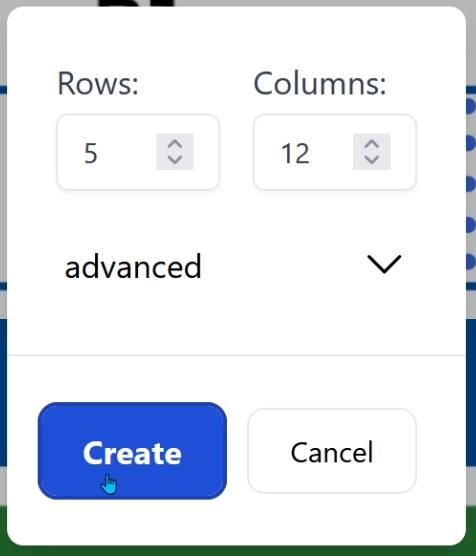
\includegraphics[width=0.4\textwidth]{pics/grid-tool.png}
    \caption{Grid-Tool Settings Modal}
    \label{fig:grid-tool-toolbar}
\end{figure}

\subsection{Conclusion}
The grid tool is designed for speed and precision when placing large quantities of seats. Its modal-based configuration, combined with interactive box selection and undoable batch insertion, makes it a powerful tool for large-scale seat placement in structured layouts.
